% !TEX root = main.tex
\documentclass[10pt, a4paper]{article}

% ── Packages ──────────────────────────────────────────────────────────────────
\usepackage[
  top=0.35in, bottom=0.35in,
  left=0.45in, right=0.45in
]{geometry}
\usepackage[dvipsnames]{xcolor}
\usepackage{hyperref}
\usepackage{graphicx}
\usepackage{titlesec}
\usepackage{enumitem}
\usepackage{array}
\usepackage{tabularx}
\usepackage{parskip}

% ── Hyperlink styling ─────────────────────────────────────────────────────────
\hypersetup{
  colorlinks=true,
  urlcolor=black,
  linkcolor=black
}

\pagestyle{empty}

% Section formatting
\titleformat{\section}
  {\normalsize\bfseries}
  {}{0em}{\MakeUppercase}
  [\vspace{-6pt}\rule{\linewidth}{0.5pt}]

\titlespacing{\section}{0pt}{6pt}{2pt}

\setlist[itemize]{noitemsep, topsep=0pt, partopsep=0pt, parsep=0pt, leftmargin=1.1em, itemsep=0pt}

\setlength{\parindent}{0pt}
\setlength{\parskip}{0pt}

% Set base font size slightly larger than 10pt default
\fontsize{10.5}{13.5}\selectfont

% ══════════════════════════════════════════════════════════════════════════════
\begin{document}

% ── HEADER ────────────────────────────────────────────────────────────────────
\noindent
\begin{minipage}[c]{0.48\textwidth}
  \raggedright
  {\fontsize{24}{28}\selectfont \textbf{YOUR NAME}}\par
  \vspace{3pt}
  {\large\itshape\color{gray} Backend Engineer $|$ API \& Scalable Systems}\par
\end{minipage}%
\hfill
\begin{minipage}[c]{0.36\textwidth}
  \raggedleft
  \begin{minipage}[c]{0.68\linewidth}
    \raggedleft
    {\small\itshape\color{gray}
      \href{mailto:your.email@example.com}{your.email@example.com}\\[3pt]
      +91\,00000\,85302\\[3pt]
      \href{https://linkedin.com/in/your-linkedin}{linkedin.com/in/your-linkedin}\\[3pt]
      \href{https://github.com/your-github}{github.com/your-github}\\
    }
  \end{minipage}%
  \hspace{0.1pt}
\begin{minipage}[c]{0.26\linewidth}
    \raggedleft
    \fboxsep=2pt\fboxrule=0.5pt
    \fbox{%
      \IfFileExists{../../assets/profile-photo.jpg}{%
        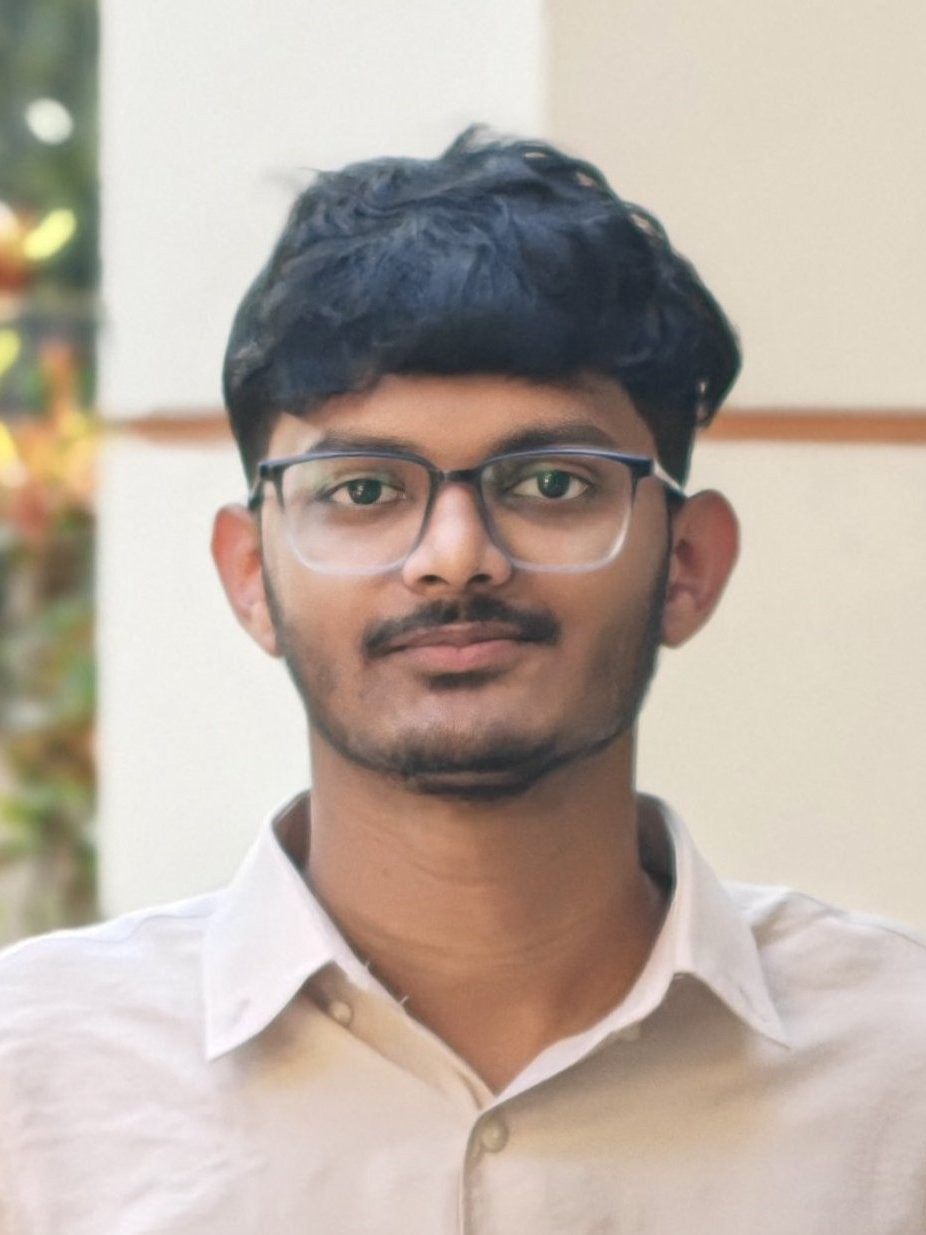
\includegraphics[height=0.75in,keepaspectratio]{../../assets/profile-photo.jpg}}{%
      \IfFileExists{../../assets/profile-photo.png}{%
        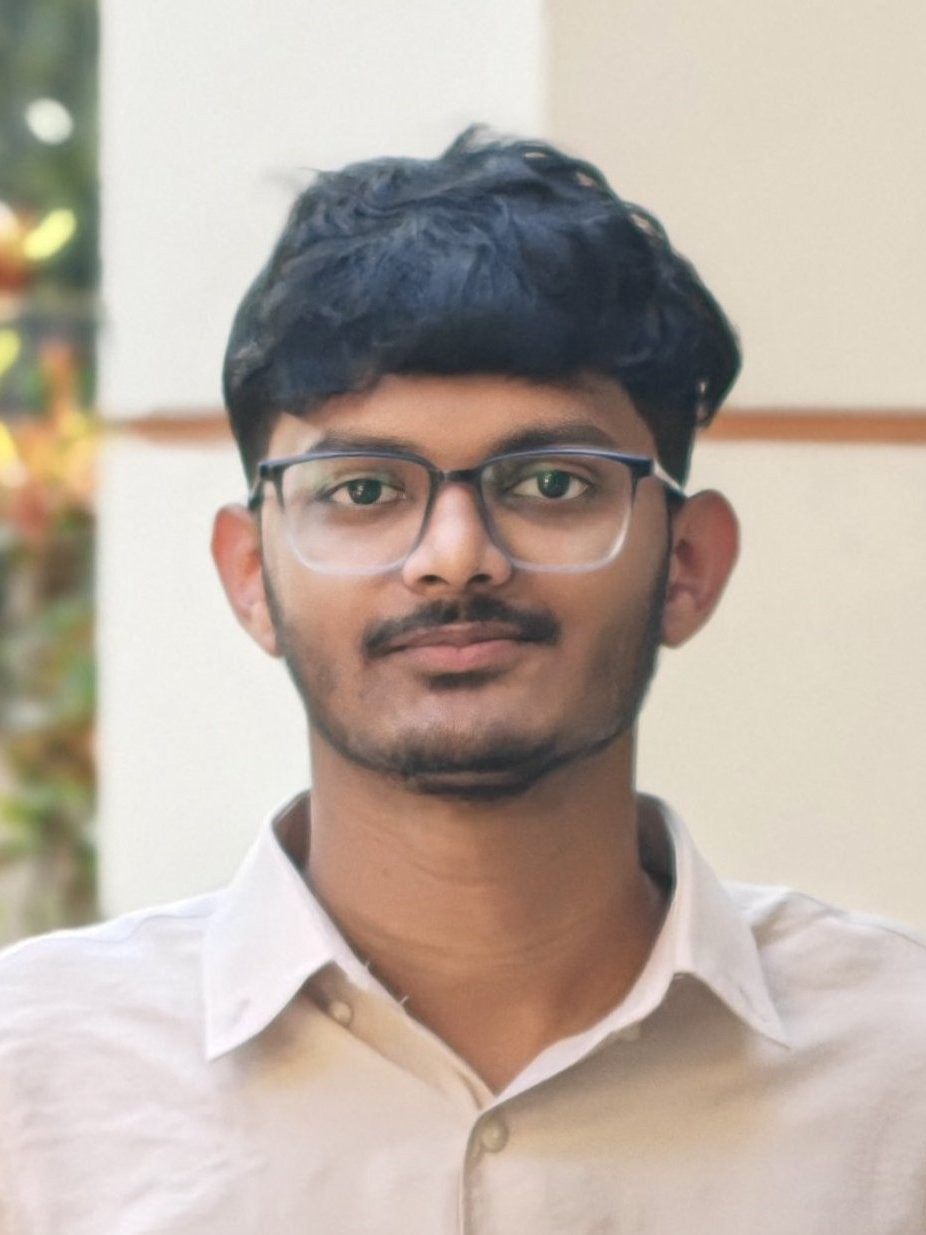
\includegraphics[height=0.75in,keepaspectratio]{../../assets/profile-photo.png}}{%
      \IfFileExists{../../assets/photo.jpg}{%
        \includegraphics[height=0.75in,keepaspectratio]{../../assets/photo.jpg}}{%
      \IfFileExists{../../assets/photo.png}{%
        \includegraphics[height=0.75in,keepaspectratio]{../../assets/photo.png}}{}}}}%
    }%
  \end{minipage}
\end{minipage}

% ── CONTENT ──────────────────────────────────────────────────────────────────
\section*{Professional Summary}

Backend Engineer specializing in Scalable Distributed Systems, RESTful API Orchestration, and Real-time Data Pipelines. Proven track record of developing production-ready architectures with 40\% efficiency gains. Proficient in Node.js, Flask, and Go, focusing on high-concurrency processing, database optimization, and automated deployment workflows.

%------------------------------------------------------------
% TECHNICAL SKILLS
%------------------------------------------------------------
\section*{Skills}

\renewcommand{\arraystretch}{1.0}
\begin{tabular}{@{} >{\bfseries}p{3.8cm} p{13cm} @{}}
Languages           & Python, Go, JavaScript \\
Backend             & Node.js, Flask, Django, Express.js, REST API Design, Microservices \\
Databases           & MongoDB, MySQL, Supabase, DB Optimization \\
Cloud/Deployment    & AWS API Gateway, Docker, DigitalOcean, Vercel, Render \\
Architecture        & Scalable Architecture, Authentication, Batch Processing \\
Operating Systems   & Linux, Windows \\
\end{tabular}

%------------------------------------------------------------
% PROJECTS
%------------------------------------------------------------
\section*{Projects}

\textbf{Certificate Generator and Verification System} \hfill \textit{Node.js, Firebase, EJS, Tailwind \quad Dec 2024} \quad \href{https://github.com/your-github/advanced-certificate-generator}{GitHub}
\begin{itemize}
\item Architected high-throughput REST APIs for bulk certificate processing of 1,000+ records with 90\% efficiency.
\item Engineered optimized database indexing and query logic ensuring low-latency data retrieval and validation.
\item Implemented secure QR-based verification enabling instant, cryptographically-linked credential validation.
\end{itemize}

\vspace{2pt}

\textbf{IRRIGO -- Smart Irrigation Platform} \hfill \textit{Next.js, Flask, Python, REST APIs \quad Oct 2024}
\begin{itemize}
\item Developed an event-driven backend integrating satellite and weather data for real-time telemetry processing.
\item Architected data-intensive RESTful services supporting 50+ concurrent agricultural monitoring scenarios.
\item Optimized agricultural water utilization by 20\% through automated decision-making and precise scheduling logic.
\end{itemize}

\vspace{2pt}

\textbf{AI-Based Smart Traffic System Using Computer Vision} \hfill \textit{Python, YOLO, Flask \quad Jan 2025}
\begin{itemize}
\item Engineered a real-time telemetry processing engine integrated with YOLO-v8 for automated signal control.
\item Optimized intersection throughput by 25\% via adaptive frequency-control and congestion analysis algorithms.
\item Architected a high-concurrency Flask backend delivering sub-200ms processing latency for edge deployment.
\end{itemize}

\vspace{2pt}

\textbf{DroidOps -- Android Device Management GUI} \hfill \textit{Tauri, React, Rust, TypeScript \quad Dec 2025} \quad \href{https://github.com/your-github/droidops}{GitHub}
\begin{itemize}
\item Architected a native-performance cross-platform GUI for ADB, reducing manual device operations by 40\%.
\item Streamlined device management via intuitive UI with optimized Rust backend command execution.
\item Integrated batch processing features for automated unit testing and environment setup.
\end{itemize}

\vspace{2pt}

\textbf{GlyphDeck -- Desktop Font Manager} \hfill \textit{Go, TypeScript, Wails \quad Nov 2025} \quad \href{https://github.com/your-github/GlyphDeck}{GitHub}
\begin{itemize}
\item Architected a high-concurrency Go application indexing 1,200+ fonts with sub-500ms retrieval latency.
\item Enhanced search and retrieval performance by 40\% through optimized custom indexing and metadata parsing.
\item Developed memory-efficient native executable approximately 25MB with native performance using Go.
\end{itemize}

%------------------------------------------------------------
% EDUCATION
%------------------------------------------------------------
\section*{Education}

\textbf{B.Tech in Computer Science and Engineering} \hfill \textbf{2022 -- 2026}\\
Mar Baselios Christian College of Engg. \& Tech., Kuttikkanam \hfill APJ Abdul Kalam Technological University

%------------------------------------------------------------
% CERTIFICATIONS
%------------------------------------------------------------
\section*{Certifications}

\renewcommand{\arraystretch}{1.0}
\begin{tabular}{@{} p{7.8cm} p{6.5cm} p{2.5cm} @{}}
\textbf{Certificate}                  & \textbf{Issuer}              & \textbf{Year} \\[1pt]
Programming with Python               & Python Institute OpenEDG   & 2024 \\
Amazon API Gateway for Serverless     & AWS Training                 & Jun 2025 \\
Ubuntu Linux Professional Certificate & Canonical                    & Nov 2025 \\
\end{tabular}

%------------------------------------------------------------
% ACHIEVEMENTS
%------------------------------------------------------------
\section*{Achievements}

\begin{tabular}{@{} p{9.5cm} p{8cm} @{}}
Galactic Problem Solver              & NASA Space Apps Challenge 2024 \\
Global Nominee                       & NASA Space Apps Challenge 2025 \\
\end{tabular}

%------------------------------------------------------------
% ADDITIONAL INFO
%------------------------------------------------------------
\section*{Additional Information}

\begin{tabular}{@{} >{\bfseries}p{3.8cm} p{13cm} @{}}
Areas of Interest & Backend Development, REST APIs, Microservices, Distributed Systems, Cloud Computing, Database Management, API Design, Server-Side Development \\
Languages         & English Professional, Malayalam Native \\
\end{tabular}

\end{document}